% Created 2022-04-19 Tue 06:12
% Intended LaTeX compiler: pdflatex
\documentclass[11pt]{article}
\PassOptionsToPackage{hyphens}{url}
\usepackage[utf8]{inputenc}
\usepackage[T1]{fontenc}
\usepackage{graphicx}
\usepackage{grffile}
\usepackage{longtable}
\usepackage{wrapfig}
\usepackage{rotating}
\usepackage[normalem]{ulem}
\usepackage{amsmath}
\usepackage{textcomp}
\usepackage{amssymb}
\usepackage{capt-of}
\usepackage{hyperref}
\usepackage{minted}
\def\ORGTITLE      {AFIM}
\def\ORGAUTHOR     {DP@H$_2$O}
\usepackage{minted}
\usepackage[margin=0.5in]{geometry}
\usepackage[x11names]{xcolor}
\usepackage{siunitx}
\hypersetup{linktoc=all, colorlinks=true, urlcolor=DodgerBlue4, citecolor=PaleGreen1, linkcolor=black}
\author{DP@H2O}
\date{\today}
\title{Australian Fast Ice Modelling\\\medskip
\large Grounded Icebergs}
\begin{document}

\maketitle
\tableofcontents


\section{Concept}
\label{sec:org034ad6e}

 It is understood that grounded icebergs act as a focal point for
fast ice to anchor \cite{zotero://select/items/1_6DH4IZVS}
and
 hence act as potential stabilisation platform and buttressing for polynya formation \cite{}. It is
 therefore important to understand the seasonal distribution of icebergs. It may be only a
 distribution that is needed and not exact map locations with iceberg shapes (volumes) and
 orientations. So that a model is not dynamically applying a grounded iceberg field but using the
 statistical knowledge of their distribution as an initial condition. The logic of this is based on
 model resolution and treating icebergs as islands. Another factor is that the underlying
 bathymetry on which icebergs ground is not changing on the same timescale as the
 ice-ocean-atmosphere and hence a seasonal approximation of locations will be valid over decadal
 scales. However, as the temporal scale shifts to centuries and millennia this approach will no
 longer be valid. The concentration of this work is considering temporal scales less than a century
 and hence the effort here is to work on the statistical distribution as method to gain a more
 robust methodology (dynamical) on future iterations of this work.

\subsection{Why SAR?}
\label{sec:org0550808}

\href{https://sentinels.copernicus.eu/web/sentinel/user-guides/sentinel-1-sar/overview}{Sentinel-1/2 SAR} is great at discriminating between icebergs and sea ice. Sentinel-1 gives us
sufficient resolution to see iceberg shapes down to the scale that is required of \href{https://github.com/dpath2o/AFIM}{AFIM}, which
gives the potential for us to unequivocally state which bergs are
truly grounded.

\section{Methodology}
\label{sec:org4df0190}

Topographically sea ice

Examine sequential temporal Sentinel-1/2 images and determine which icebergs are not moving. These
\uline{could} be mapped and form the prescribed field of grounded bergs for AFIM or they could form the
basis on which to determine a seasonal distribution. In beginning this effort the simplest
approach and one that will give me a better understanding of the remote sensing technology and one
aspect of the sea ice dynamics is to utilised \href{https://coastwatch.noaa.gov/cw\_html/cw\_polygon\_search.html}{NOAA's Coastwatch Polygon Search}. Look through pairs
of images. Each pair is separated by 12-days which provides nearly exact geographic domain and
aspect angle of incident Sentinel SAR images. When using NOAA's Coastwatch website it allows for
one to open up several tabs of sequential (12-day images) and 'flick' between them to see the
ocean-sea ice dynamics. In this manner I can select a pair of images to then trace the common
grounded icebergs. This should end with a grounded iceberg occupying
at least one pixel.

After reviewing a number of images from NOAA's Coastwatch webpage, I
decided to make a year's animation from the NOAA processed SAR data
that are comprised of 28 images for each region that I called: Cape
Darnley, Mawson Coast and Prydz Bay. The animations are displad
in-line with the text below and indicate a number of probable
grounded icebergs in each region. 

\begin{itemize}
\item Cape Darnley (high resolution)
\url{../GRAPHICAL/grounded\_icebergs/preliminary\_work/CapeDarnley\_NOAA\_CoastWatch\_Animation\_2019-2020.gif}
\item Mawson Coast (high resolution)
\url{../GRAPHICAL/grounded\_icebergs/preliminary\_work/MawsonCoast\_NOAA\_CoastWatch\_Animation\_2019-2020.gif}
\item Prydz Bay (lower resolution)
\url{../GRAPHICAL/grounded\_icebergs/preliminary\_work/PrydzBay\_NOAA\_CoastWatch\_Animation\_2019-2020.gif}
\end{itemize}

\section{Current Image Pairs}
\label{sec:orga5bca97}

I choose the following two images based on the time-of-year,
overlapping regions (Cape Darnley and Prydz Bay) and contrast of
likely grounded icebergs and sea ice / ocean.  

\subsubsection{High Resolution}
\label{sec:org280ade3}
\begin{itemize}
\item image 1
\begin{center}
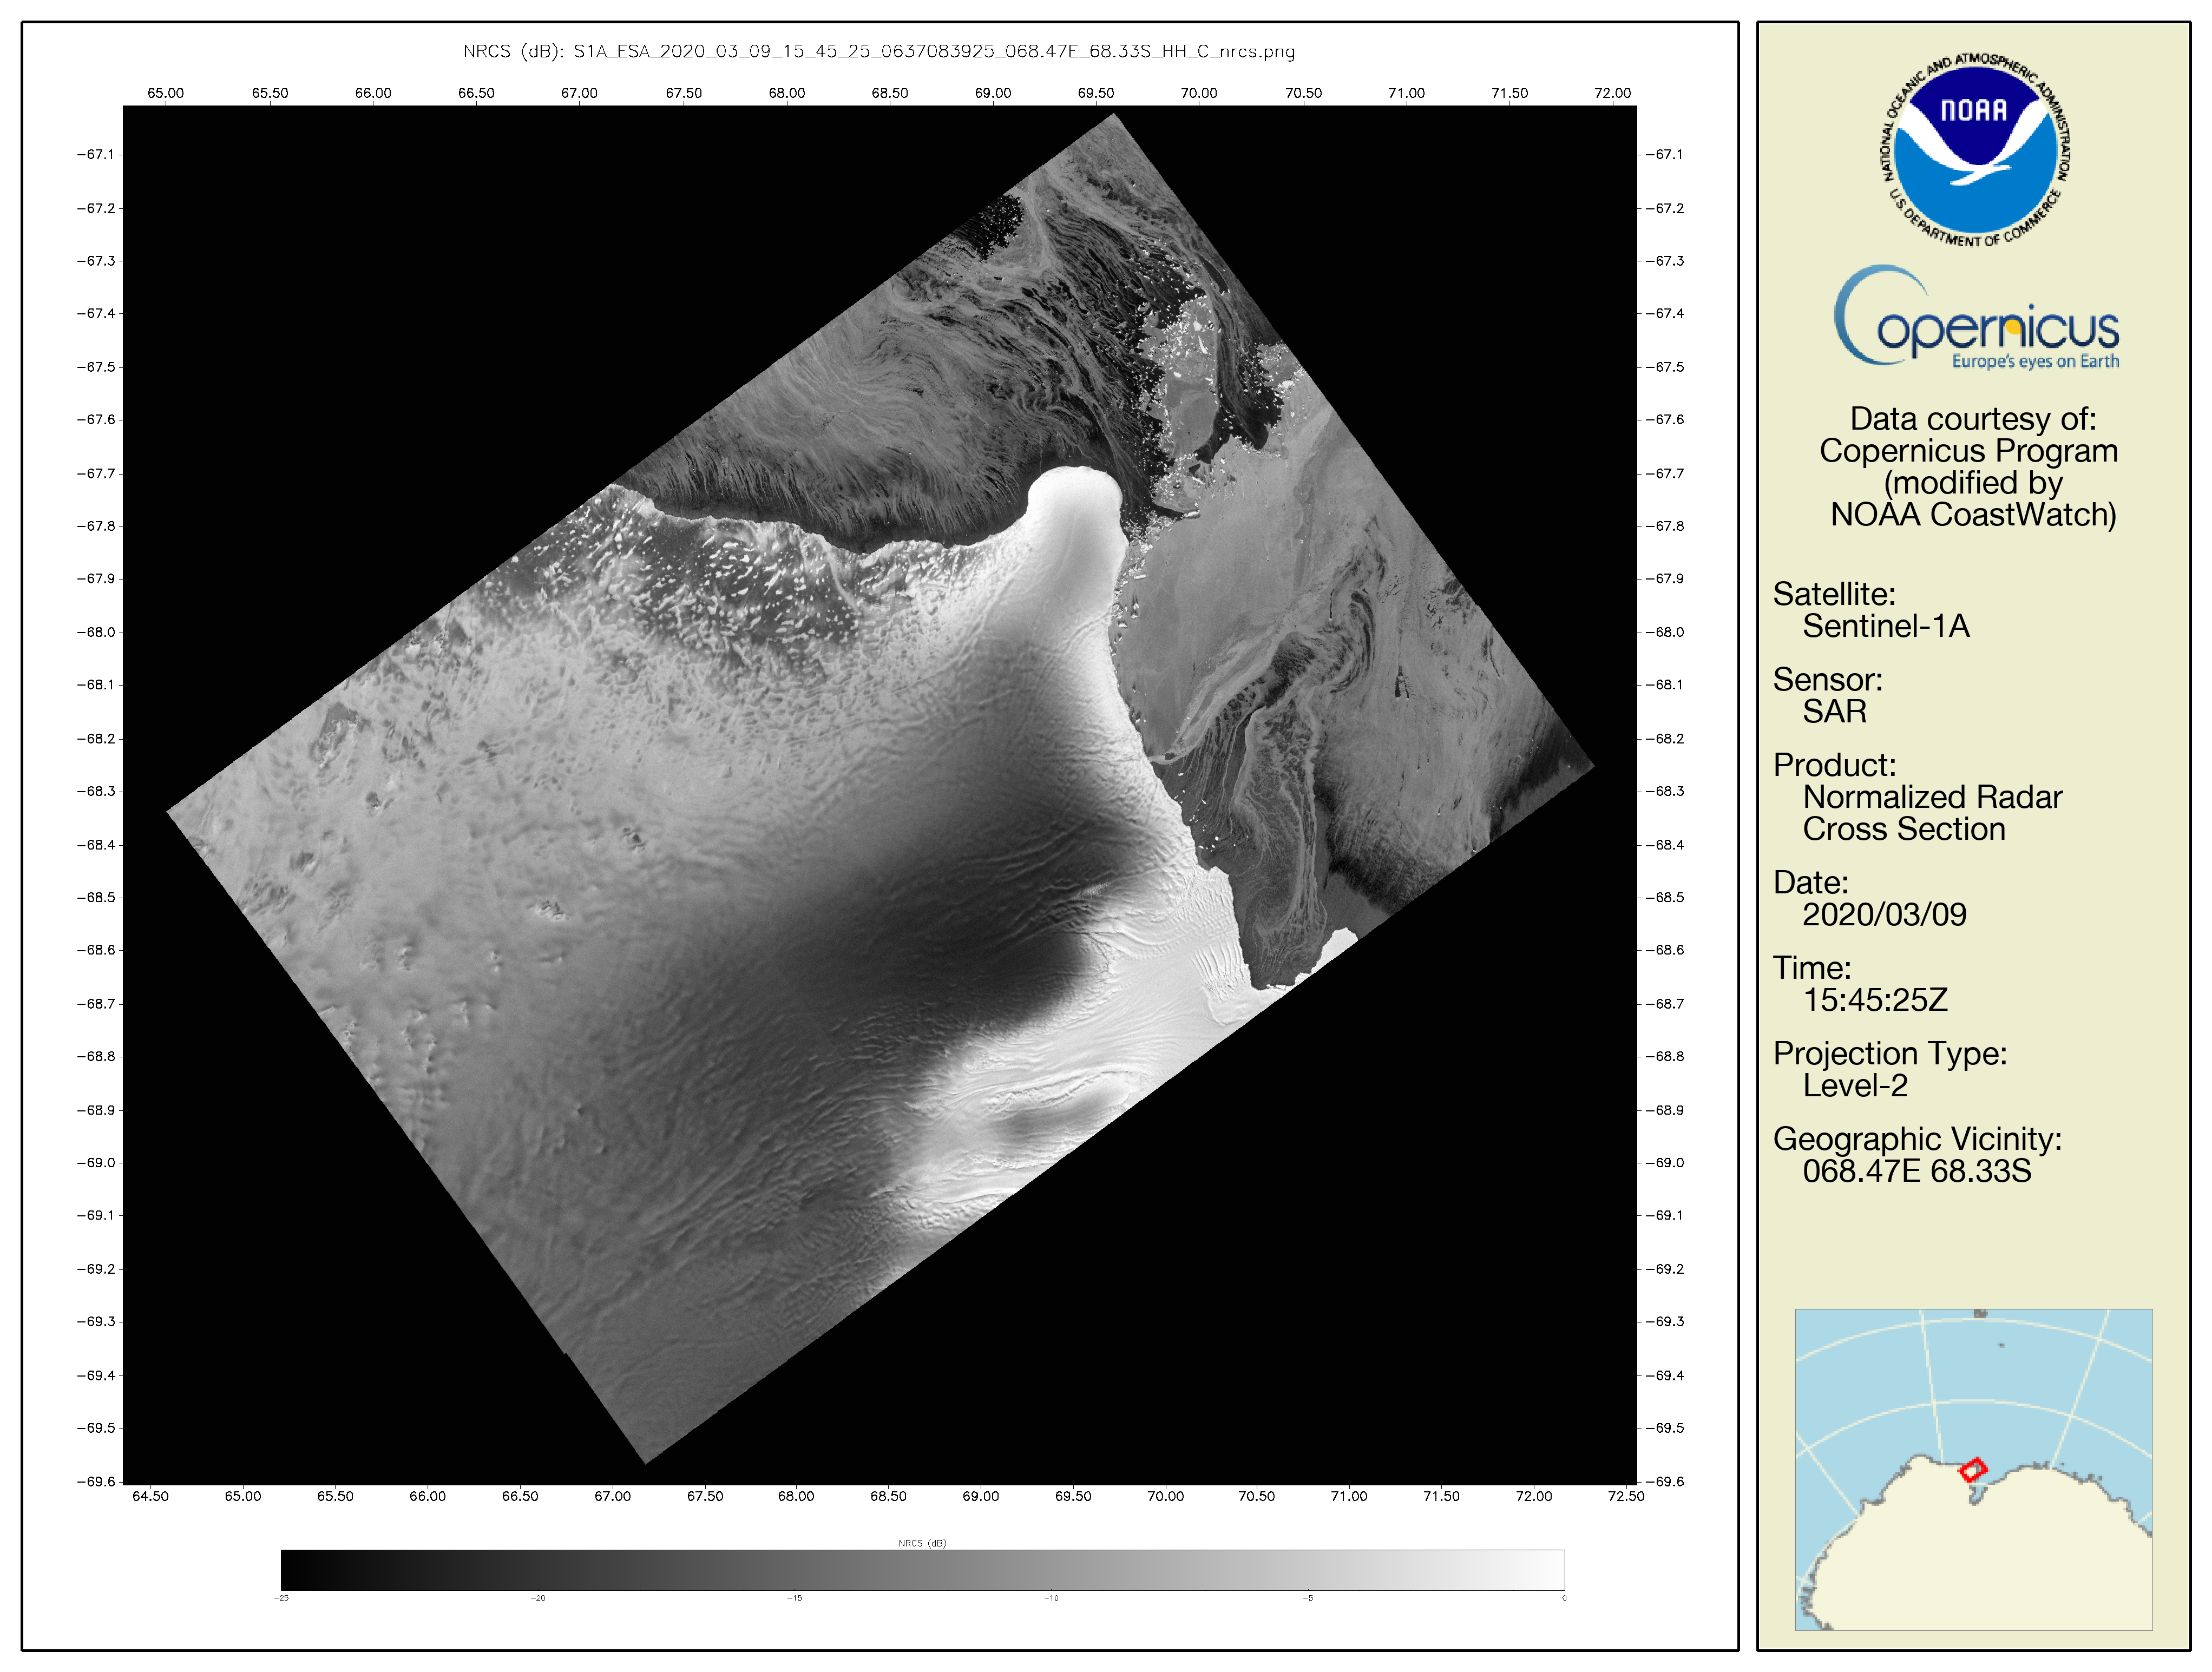
\includegraphics[width=15cm]{../GRAPHICAL/grounded_icebergs/preliminary_work/CapeDarnley/S1A_ESA_2020_03_09_15_45_25_0637083925_068.47E_68.33S_HH_C_nrcs_level2.png}
\end{center}
\item image 2
\begin{center}
\includegraphics[width=15cm]{../GRAPHICAL/grounded_icebergs/preliminary_work/CapeDarnley/S1A_ESA_2020_03_21_15_45_26_0638120726_068.47E_68.33S_HH_C_nrcs_level2.png}
\end{center}
\end{itemize}
\subsubsection{Low Resolution}
\label{sec:org72ce55e}
\begin{itemize}
\item image 1
\begin{center}
\includegraphics[width=15cm]{../GRAPHICAL/grounded_icebergs/preliminary_work/PrydzBay/S1A_ESA_2020_03_13_15_12_43_0637427563_074.19E_68.08S_HH_C_nrcs_level2.png}
\end{center}
\item image 2
\begin{center}
\includegraphics[width=15cm]{../GRAPHICAL/grounded_icebergs/preliminary_work/PrydzBay/S1A_ESA_2020_03_25_15_12_43_0638464363_074.18E_68.08S_HH_C_nrcs_level2.png}
\end{center}
\end{itemize}


\section{Methods of Downloading Level 1 Sentinel SAR Data}
\label{sec:org06b28da}

As I ran into delays with python method I chose to download the data
from RDI/CDASO. The delay with the python method was that the online
archive was not making the data available at 24 or 48 or 72 hours
after the initial request.

\subsection{Download the image pair via python}
\label{sec:org1a73d0b}

\begin{enumerate}
\item Before downloading the python environment needs to be loaded to recognise the required python
modules -- assuming local buffer configuration
\item Also it very beneficial to understand \href{https://sentinelsat.readthedocs.io/en/master/api\_overview.html}{python module sentinalsat} , which in my particular case
I've opted to use \url{file:///Users/dpath2o/.netrc} file to store my sensitive login information
\item One must create a \href{https://geojson.org}{GeoJSON} file and edit this code to work on that file
\item For this particular instance (example) I'm using \url{file:///Users/dpath2o/PHD/etc/Mawson.geojson}
\begin{minted}[breaklines=true,breakanywhere=true,frame=single]{python}
#LIBRARY IMPORT
import os
import pprint
from sentinelsat import SentinelAPI, read_geojson, geojson_to_wkt
# HARDWIRED PARAMETERS -- need a better way of putting a passocde in here
Dbase  = os.path.join('/','Users','dpath2o')
Ddata  = os.path.join(Dbase,'DATA','Satellite','Sentinel','MawsonCoast')
Fgeoj  = os.path.join(Dbase,'PHD','etc','Mawson.geojson')
# The geojson file makes this a bit transferable and easier to setup different regions
# later on, but it requires that sentinalsat can use and we use to functions from the
# sentinelsat API
ftprt  = geojson_to_wkt(read_geojson(Fgeoj))
# Hi-Res IMAGE 1 -- using a narrow 
qkwar  = {'platformname': 'Sentinel-1',
	  'producttype': 'GRD',
	  'date': ('2019-02-19T15:40:00.000Z','2019-02-19T15:50:00.000Z' ),
	  'instrumentshortname': 'SAR-C SAR',
	  'sensoroperationalmode': 'EW'}
apic     = SentinelAPI(None, None, 'https://scihub.copernicus.eu/dhus')
Qresults = apic.query(ftprt,**qkwar)
Qdf      = apic.to_dataframe(Qresults)
for f in Qresults:
    print('Filename {}'.format(Qdf.title[f]))
    online_test = apic.get_product_odata(f)
    if not online_test['Online']:
	print('{} is NOT online ... skipping'.format(Qdf.title[f]))
	continue
    apic.download(f,Ddata)
# Hi-Res IMAGE 2 -- only changing the datetime to 12 days later as this will give us the exact
#            same image
qkwar  = {'platformname': 'Sentinel-1',
	  'producttype': 'GRD',
	  'date': ('2019-03-15T15:40:00.000Z','2019-03-15T15:50:00.000Z' ),
	  'instrumentshortname': 'SAR-C SAR',
	  'sensoroperationalmode': 'EW'}
apic     = SentinelAPI(None, None, 'https://scihub.copernicus.eu/dhus')
Qresults = apic.query(ftprt,**qkwar)
Qdf      = apic.to_dataframe(Qresults)
for f in Qresults:
    print('Filename {}'.format(Qdf.title[f]))
    online_test = apic.get_product_odata(f)
    if not online_test['Online']:
	print('{} is NOT online ... skipping'.format(Qdf.title[f]))
	continue
apic.download(f,Ddata)
# Low-Res IMAGE 1 -- using a narrow 
qkwar  = {'platformname': 'Sentinel-1',
	  'producttype': 'GRD',
	  'date': ('2019-02-26T15:30:00.000Z','2019-02-26T15:40:00.000Z' ),
	  'instrumentshortname': 'SAR-C SAR',
	  'sensoroperationalmode': 'EW'}
apic     = SentinelAPI(None, None, 'https://scihub.copernicus.eu/dhus')
Qresults = apic.query(ftprt,**qkwar)
Qdf      = apic.to_dataframe(Qresults)
for f in Qresults:
    print('Filename {}'.format(Qdf.title[f]))
    online_test = apic.get_product_odata(f)
    if not online_test['Online']:
	print('{} is NOT online ... skipping'.format(Qdf.title[f]))
	continue
    apic.download(f,Ddata)
# Low-Res IMAGE 2 -- only changing the datetime to 12 days later as this will give us the exact
#            same image
qkwar  = {'platformname': 'Sentinel-1',
	  'producttype': 'GRD',
	  'date': ('2019-03-10T15:30:00.000Z','2019-03-10T15:40:00.000Z' ),
	  'instrumentshortname': 'SAR-C SAR',
	  'sensoroperationalmode': 'EW'}
apic     = SentinelAPI(None, None, 'https://scihub.copernicus.eu/dhus')
Qresults = apic.query(ftprt,**qkwar)
Qdf      = apic.to_dataframe(Qresults)
for f in Qresults:
    print('Filename {}'.format(Qdf.title[f]))
    online_test = apic.get_product_odata(f)
    if not online_test['Online']:
	print('{} is NOT online ... skipping'.format(Qdf.title[f]))
	continue
apic.download(f,Ddata)
\end{minted}
\end{enumerate}

\subsection{Download the image pair via \href{file:///Users/dpath2o/PHD/admin/computing.org}{RDI\textsubscript{CDASO}}}
\label{sec:orgb81ca0a}
\subsection{Download the image pair via \href{https://apps.sentinel-hub.com/eo-browser/?zoom=10\&lat=41.9\&lng=12.5\&themeId=DEFAULT-THEME\&toTime=2022-04-13T20\%3A52\%3A55.350Z}{SentinelHub}}
\label{sec:org9d03bcf}

\section{Rasterise Sentinel Level 1 SAR Data}
\label{sec:orgeb29db6}

Sentinel Level 1 SAR Data is not provided in a geo-referenced
projection and hence to manually analyse the data with respect to grounded
icebergs it is necessary to re-project (map) the data. As geotiffs
can be vectorised (i.e. each pixel can be accessed for information)
and geographical/mapping information travels with the file
(header/metadata) then this is the obvious file format to rasterise
the SAR Level 1 data. There are number of ways to do this and some
toolboxes that could be explored for future automation.

One method via python is provided below as wellas another method,
the one that I used to rasterise the four separate SAR Level 1
sweeps, via Sentinal SNAP toolbox.

I did some background reading on SAR and the Amery Ice Shelf calving event of
2019 — the later being something I observed while looking through NOAA
Coastwatch images. On Monday, after SentinelHub still had not released
the products, I decided to go through our previous email discussion in
August of last year. I found that Glenn had given me access to
RDSI/CDASO, which I had completely forgot about. By that stage on
Monday I had identified these three domains (hi-res CD, hi-res MC,
low-res PB) and took the liberty to download the corresponding data
from RDSI/CDASO. By then it was Tuesday and I had a crack at
processing a pair of images using the code provided here. However,
after several attempts and variations I only get a blank (black) image
as a result, albeit a 1.5GB blank image. As I wanted to have a better
understanding of the tif (data) I found this little chestnut , as well
as these two bodies of work: ASF and GMTSAR. The later describe
working with raw interferometry SAR (InSAR) sentinel-1 and an example
of Larsen Ice Shelf (which is a link at the bottom of that page, but
be warned the download is 4GB). 

\subsection{Rasterise via python}
\label{sec:orgb418e77}

Rasterisation is similarly performed using pre-configured python environment that has python
module \href{https://rasterio.readthedocs.io/en/latest/}{rasterio}

\begin{minted}[breaklines=true,breakanywhere=true,frame=single]{python}
import rasterio
from rasterio.warp import calculate_default_transform, reproject, Resampling
import glob
import os
import zipfile
import tempfile
Dbase  = os.path.join('/','Users','dpath2o')
Ddata  = os.path.join(Dbase,'DATA','Satellite','Sentinel','MawsonCoast')
Dproc  = os.path.join(Ddata,'proc')
if not os.path.exists(Dproc): os.makedirs(Dproc)
Fnames = glob.glob("{}/*.zip".format(Ddata))
CRS    = 'EPSG:3031'
for f in Fnames:
    DFin,Fin = os.path.split(f)
    Ftmp     = os.path.join(Dproc,"{}.SAFE".format(os.path.splitext(Fin)[0]))
    Fout     = os.path.join(Dproc,'{}.tif'.format(os.path.splitext(Fin)[0]))
    with zipfile.ZipFile(f, 'r') as zip_ref:
	zip_ref.extractall(Dproc)
    with rasterio.open(Ftmp) as src:
	gcps,gcp_crs = src.gcps
	xfrm,w,h     = calculate_default_transform( gcp_crs , CRS , src.width , src.height ,  gcps=gcps )
	kwargs       = src.meta.copy()
	kwargs.update({ 'crs'      : CRS,
			'transform': xfrm,
			'width'    : w,
			'height'   : h,
			'driver'   : 'GTIFF',
			'compress' : 'lzw',
			'NBITS'    : 10 })
	with rasterio.open(Fout, 'w', **kwargs) as dst:
	    for i in range(1, src.count + 1):
		reproject( source        = rasterio.band(src, i),
			   destination   = rasterio.band(dst, i),
			   src_transform = src.transform,
			   src_crs       = src.crs,
			   dst_transform = xfrm,
			   dst_crs       = CRS,
			   resampling    = Resampling.nearest)
\end{minted}

\subsection{Rasterise via \href{https://step.esa.int/main/download/snap-download/}{SNAP}}
\label{sec:orgf15dc9c}

\begin{enumerate}
\item Follow the directions for downloading and installing SNAP
\item Load zip files (image pairs) into SNAP
\item Select Radar -> Geometric -> Elipsoid Correction -> Geolocation-Grid
\item Use EPSG:3031 as the new projection
\end{enumerate}

\subsection{Use \href{https://www.gimp.org}{GIMP} for layering and merging}
\label{sec:orgffd28e8}

In the first instance two \texttt{merged} figures were created and can be
found on my Google hard drive: \href{https://drive.google.com/file/d/12rBVi-qdNDChf6J3M1tdehBGgWYahPi4/view?usp=sharing}{Cape Darnley} (high resolution, \textasciitilde{}100MB) and
\href{https://drive.google.com/file/d/1n-bSFUpUhzv7L2\_1GMLRy7NRP9oeFEXM/view?usp=sharing}{Prydz Bay} (low resolution, \textasciitilde{}50MB). These two PNGs were merged in GIMP from
their source geotiff files where are available below.

\subsubsection{\href{https://drive.google.com/file/d/1n39IWX\_VriVqEc3Dnr65nqIvBzBSVOhi/view?usp=sharing}{Cape Darnley (higher resolution) geotiff 09 Mar 2020 (\textasciitilde{}3GB)}}
\label{sec:org5bfc6e1}

\subsubsection{\href{https://drive.google.com/file/d/1n7ltcEQMj62ggmRoHuCI3\_toXb4tI65B/view?usp=sharing}{Cape Darnley (higher resolution) geotiff 21 Mar 2020 (\textasciitilde{}3GB)}}
\label{sec:org30509fd}

\subsubsection{\href{https://drive.google.com/file/d/1n91zwi\_NVX\_pkzerxvoOw9oGFZ-ypAWP/view?usp=sharing}{Prydz Bay (lower resolution) geotiff 13 Mar 2020 (\textasciitilde{}1GB)}}
\label{sec:orgd2d6a72}

\subsubsection{\href{https://drive.google.com/file/d/1nHceOG3D\_eweceIcVhg6Ex5nviDYZ09l/view?usp=sharing}{Prydz Bay (lower resolution) geotiff 25 Mar 2020 (\textasciitilde{}1GB)}}
\label{sec:org58191aa}
\end{document}
